\documentclass[12pt,fleqn,answers]{exam}
\usepackage{pifont}
\usepackage{dingbat}
\usepackage{amsmath,amssymb}
\usepackage{epsfig}
\usepackage[colorlinks=true,linkcolor=black,anchorcolor=black,citecolor=black,filecolor=black,menucolor=black,runcolor=black,urlcolor=black]{hyperref}
\usepackage[letterpaper, margin=0.75in]{geometry}
\addpoints
\boxedpoints
\pointsinmargin
\pointname{pts}

\usepackage{pdfpages}
\usepackage[final]{microtype}
\usepackage[american]{babel}
\usepackage[T1]{fontenc}
\usepackage{fourier}
\usepackage{isomath}
\usepackage{upgreek,amsmath}
\usepackage{amssymb}

\newcommand{\dotprod}{\, {\scriptzcriptztyle
    \stackrel{\bullet}{{}}}\,}

\newcommand{\reals}{\mathbf{R}}
\newcommand{\lub}{\mathrm{lub}} 
\newcommand{\glb}{\mathrm{glb}} 
\newcommand{\complex}{\mathbf{C}}
\newcommand{\dom}{\mbox{dom}}
\newcommand{\range}{\mbox{range}}
\newcommand{\cover}{{\mathcal C}}
\newcommand{\integers}{\mathbf{Z}}
\newcommand{\vi}{\, \mathbf{i}}
\newcommand{\vj}{\, \mathbf{j}}
\newcommand{\vk}{\, \mathbf{k}}
\newcommand{\bi}{\, \mathbf{i}}
\newcommand{\bj}{\, \mathbf{j}}
\newcommand{\bk}{\, \mathbf{k}}
\newcommand{\dist}{\, \mathrm{dist}}
\DeclareMathOperator{\Arg}{\mathrm{Arg}}
\DeclareMathOperator{\Ln}{\mathrm{Ln}}
\newcommand{\imag}{\, \mathrm{i}}

\usepackage{xcolor}
\shadedsolutions
\definecolor{SolutionColor}{rgb}{0.95,0.95,0.95}

\usepackage{graphicx}
\newcommand\AM{{\sc am}}
\newcommand\PM{{\sc pm}}
     
%\usepackage{twemojis}
\newcommand{\quiz}{6}
\newcommand{\term}{Spring}
\newcommand{\due}{9:55 \AM}
\newcommand{\class}{MATH 102}
\begin{document}
\large
\vspace{0.1in}
\noindent\makebox[3.0truein][l]{\textbf{\class, \term \/ \the\year}}
\textbf{Name:} \hrulefill \\
\noindent \makebox[3.0truein][l]{\textbf{In class work \quiz}}
\textbf{Row and Seat}:\hrulefill\\
\vspace{0.1in}


\noindent  In class work  \quiz\/  has questions 1 through  \numquestions \/ with a total of  \numpoints\/  points.   
 This assignment is due at the end of the class period (\due).

\vspace{0.1in}


\begin{questions} 

  \question Find the \emph{vertex} of each parabola

  \begin{parts}

    \part[2] $y - 8 = x^2$

    \begin{solution}[1.5in] Matching $y - 8 = x^2$ to $y - k = a (x-h)^2$
      gives $k=8, h=0$, and $a=1$.  So the vertex is the point $(0,8)$.

    \end{solution}

    \part[2] $y - 8 = \sqrt{2} (x + 2)^2$

    \begin{solution}[1.5in] Matching $y - 8 = \sqrt{2} (x + 2)^2$ to $y - k = a (x-h)^2$
      gives $k=8, h=-2$, and $a=\sqrt{2}$.  
      So the vertex is the point $(-2,8)$.


    \end{solution}

        \part[2] $y=2 {{x}^{2}}-28 x+103$

   
    \begin{solution}[1.5in] Matching $y=2 {{x}^{2}}-28 x+103$ to
      $y=a x^2 + b x + c$ gives $a=2,b=-28$, and $c=103$. The 
      vertex  is the point
      \begin{equation}
        \left(-\frac{b}{2 a}, c - \frac{b^2}{4 a}\right) = 
        \left(-\frac{-28}{2 \times 2}, 103 - \frac{(-28)^2}{4 \times 2}\right) = 
        \left(7, 5 \right).
      \end{equation}
    \end{solution}

    \part[2] $y=3 (x-2)(x-4)$
    \begin{solution} To match $y=3 (x-2)(x-4)$ to $y=a x^2 + b x + c$,
      we need to expand (use FOIL) $y=3 (x-2)(x-4)$. We have
      \begin{equation*}
          y = 3 (x-2)(x-4) = 3(x^2 -6 x + 8) = 3 x^2 - 18 x + 24.
      \end{equation*}
      So $a=3, b=-18$, and $c=24$. The 
      vertex  is the point
      \begin{equation*}
        \left(-\frac{b}{2 a}, c - \frac{b^2}{4 a}\right) = 
        \left(-\frac{-18}{2 \times 3}, 24 -\frac{(-18)^2}{4 \times 3} \right) =
        \left( 3, -3 \right).
      \end{equation*}
    \end{solution}


  \end{parts}

\end{questions}
%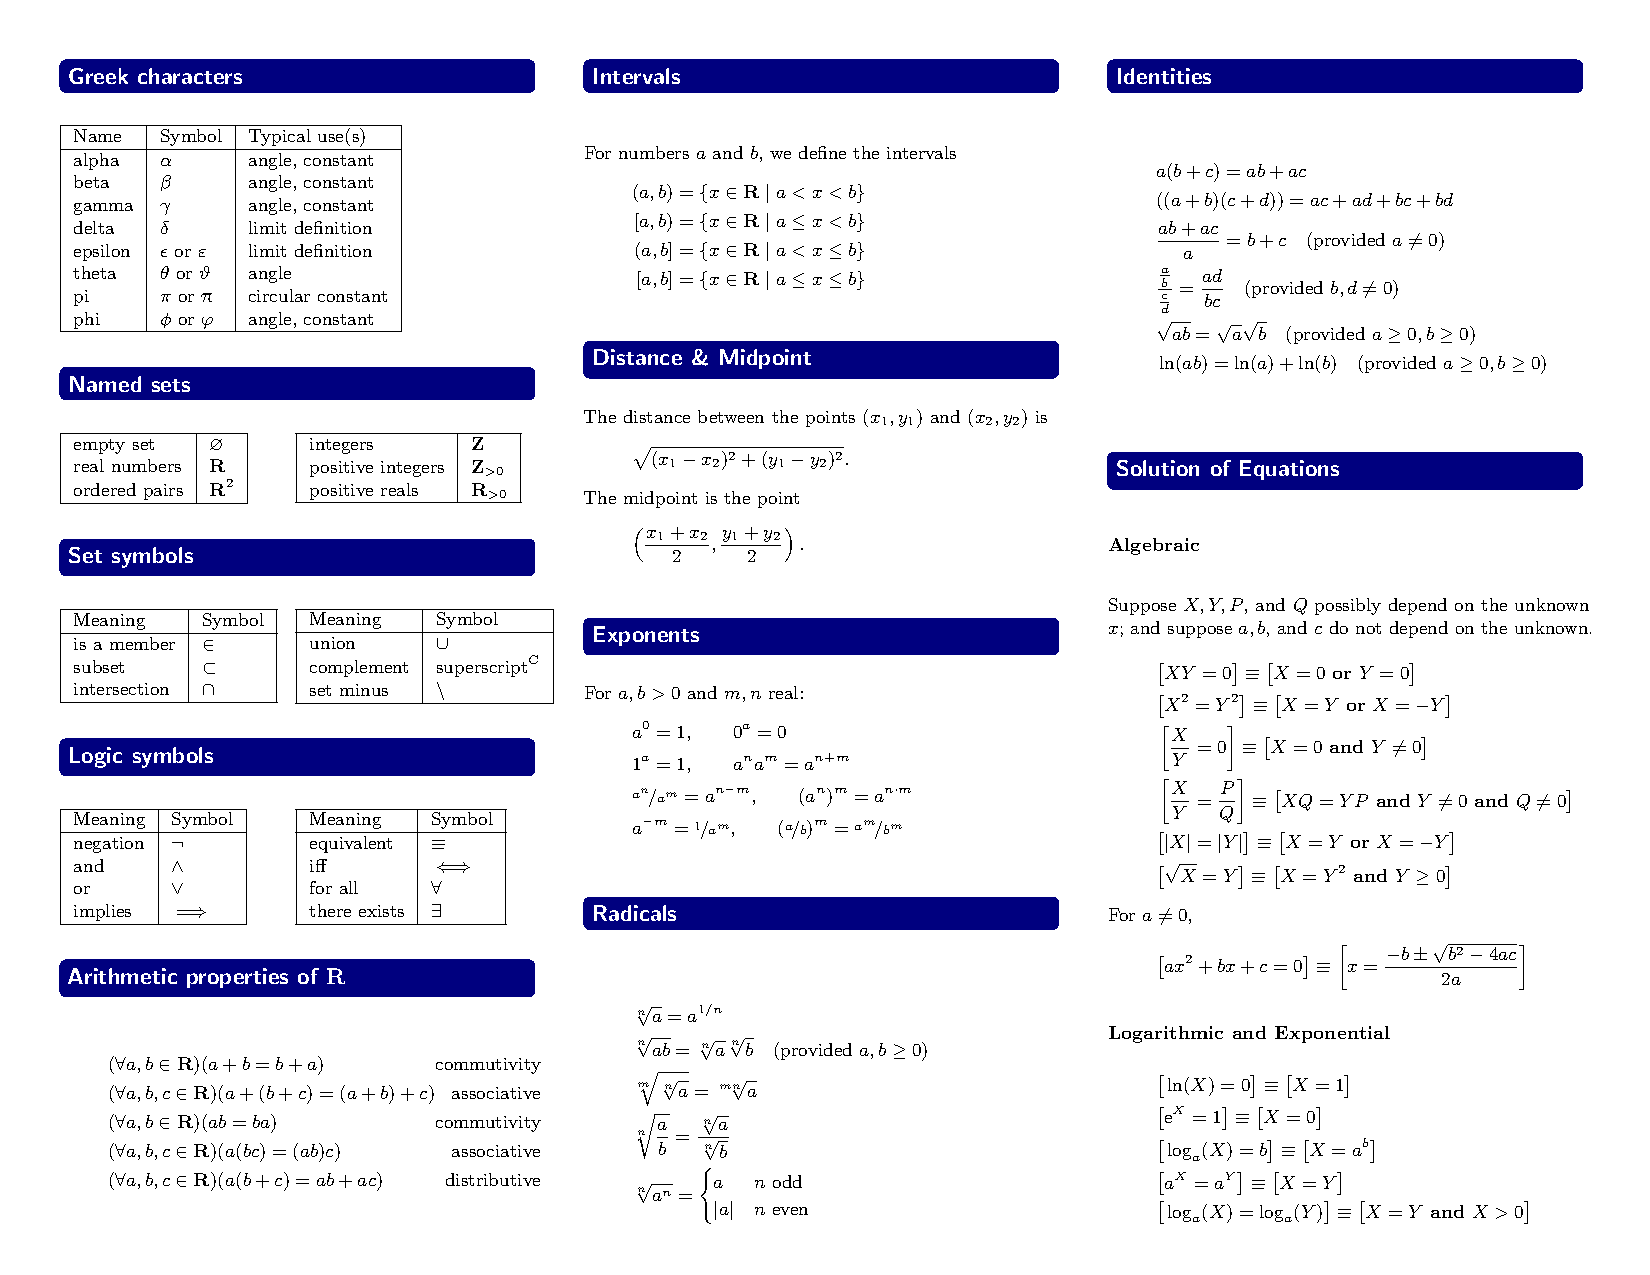
\includepdf[pages=-]{college-algebra-quick-reference.pdf}
\end{document}
